\documentclass[final,12pt]{article}
\usepackage{amsmath}
\usepackage{amssymb}
\usepackage{latexsym}
\usepackage{mathtools}
\usepackage[margin=1in]{geometry}
\usepackage[polish,english]{babel}
\usepackage[utf8]{inputenc}
\usepackage[T1]{fontenc}

\usepackage{url}
\usepackage{xspace}
\usepackage[pdftex]{graphicx}
\usepackage[pdftex]{color}

\usepackage{adjustbox}


% \definecolor{azure}{rgb}{0.0, 0.5, 0.0}
% \definecolor{processblue}{cmyk}{0.96,0,0,0}

\DeclarePairedDelimiter\abs{\lvert}{\rvert}%
\DeclarePairedDelimiter\norm{\lVert}{\rVert}%
\DeclarePairedDelimiter\set{\{}{\}}%
\DeclarePairedDelimiter\tuple{\langle}{\rangle}%

% Swap the definition of \abs* and \norm*, so that \abs
% and \norm resizes the size of the brackets, and the 
% starred version does not.
\makeatletter
\let\oldabs\abs
\def\abs{\@ifstar{\oldabs}{\oldabs*}}
%
\let\oldnorm\norm
\def\norm{\@ifstar{\oldnorm}{\oldnorm*}}
%
\let\oldset\set
\def\set{\@ifstar{\oldset}{\oldset*}}
%
\let\oldtuple\tuple
\def\tuple{\@ifstar{\oldtuple}{\oldtuple*}}
%
\makeatother
%




\begin{document}
\setlength{\parindent}{0pt}
\noindent

{\bf Teoria informacji 2023/24. Kolokwium -- Zadanie 2}

Andrzej Radzimiński, ar429586
\\

\ \\

\newcommand{\ot}{\frac{1}{3}}
\newcommand{\twt}{\frac{2}{3}}

\renewcommand*{\arraystretch}{1.5}

% Przekształcając równoważnie:
Chcemy udowodnić:
\begin{equation}
	I(f(x) ; g(y) | z) \leq I(x ; y | z),
\end{equation}
równoważnie:
$$
	0 \leq I(x ; y | z) - I(f(x) ; g(y) | z).
$$

Pokażę, że:
\begin{multline}
	I(x ; y | z) - I(f(x) ; g(y) | z) = \\
	I(x ; y | g(x), g(y), z) +
	I(g(y) ; x | f(x), z) +
	I(f(x) ; y | g(y), z).
\end{multline}
Jako, że każdy element po lewej stronie równania $(2)$ jest nieujemny (``joint conditional entropy'' oraz ``conditional mutual information'' są zawsze nieujemne), to dowiedzie do $(1)$.

\subsection*{Dowód:}

Dowód "przez obrazek":

\begin{figure}[ht!]
	\centering
	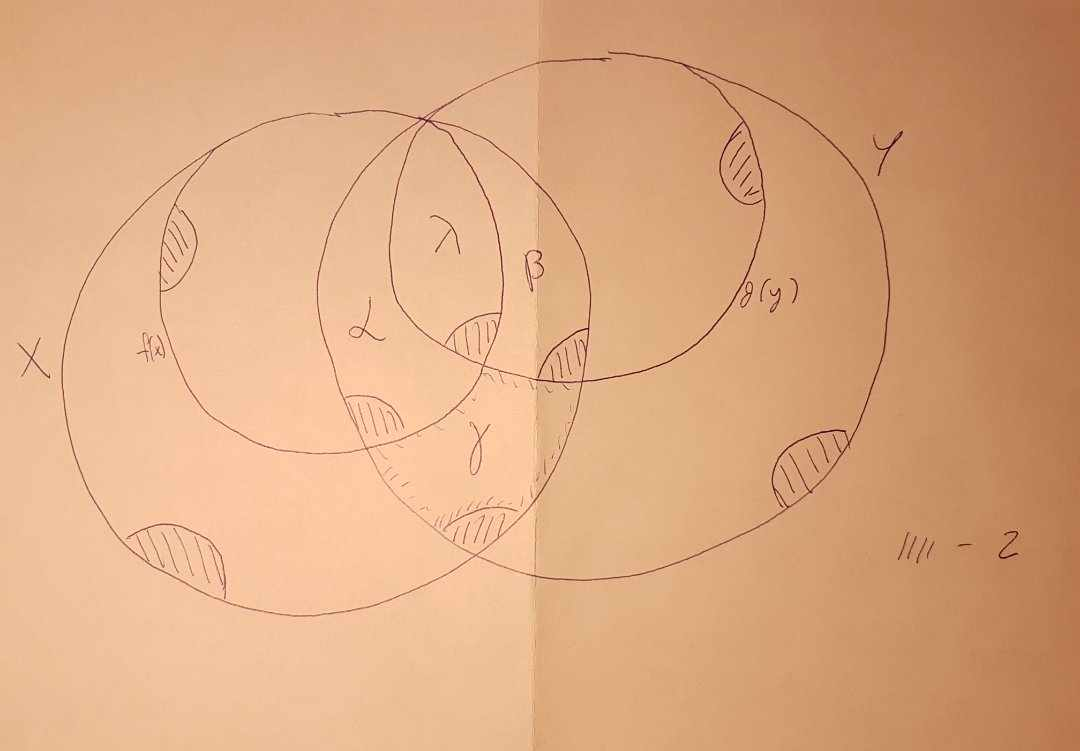
\includegraphics[width=160mm]{obrazek.jpg}
	% \caption{A simple caption \label{overflow}}
\end{figure}

\newpage
\textbf{Legenda:}

\begin{itemize}
	\item Duże kółka odpowiadają odpowiednio $x$ i $y$.
	\item Małe kółka (wewnętrzne) odpowiadają odpowiednio $f(x)$ i $f(x)$.
	\item Zakreskowane części odpowiadają zmiennej $z$ (fragment $z$ niezależny od $x$, $y$ został pominięty dla czytelności).
	\item $\alpha, \beta, \gamma, \lambda$ reprezentują najmniejsze obszary w których się zawierają (bez zakreskowanych obszarów).
\end{itemize}

\textbf{Wyjaśnienie:}

Wiadomo, że $H(f(x) | x) = 0$, a więc $f(x)$ może został w pełni zawarte na obrazku wewnątrz $x$ (analogicznie dla $y$).

Teraz możemy zdefiniować $\alpha, \beta, \gamma, \lambda$:
\begin{itemize}
	\item $\lambda = I(f(x) ; g(y) | z)$
	\item $\gamma = I(x ; y | f(x), g(y), z)$
	\item $\alpha = I(f(x) ; y | g(y), z)$
	\item $\beta = I(g(y) ; x | f(x), z)$
\end{itemize}

Jednocześnie zachodzi:
$$
	I(x; y|z) = \alpha + \beta + \gamma + \lambda,
$$
oraz
$$
	I(f(x) ; g(y) | z) = \lambda,
$$
z czego wynika:
\begin{multline*}
	I(x ; y | z) - I(f(x) ; g(y) | z) = \alpha + \beta + \gamma = \\
	I(f(x) ; y | g(y), z) + I(g(y) ; x | f(x), z) + I(x ; y | f(x), g(y), z).
\end{multline*}
Równanie to jest tym samym równaniem co $(2)$, co kończy dowód.

% $$
% H(f(x) , z) + H(g(y) , z) - H(f(x), g(y) , z) - H(z) \leq
% H(x , z) + H(y , z) - H(x, y , z) - H(z)
% $$
% $$
% H(f(x) , z) + H(g(y) , z) - H(f(x), g(y) , z) \leq
% H(x , z) + H(y , z) - H(x, y , z)
% $$
% $$
% H(f(x) , z) + H(g(y) , z) + H(x, y , z) \leq
% H(x , z) + H(y , z) + H(f(x), g(y) , z)
% $$


\end{document}